% Chapter 1

\chapter{Parallel in-situ analytics} % Main chapter title

\label{Chapter7} % For referencing the chapter elsewhere, use \ref{Chapter1}

\lhead{Chapter 7. \emph{Parallel in-situ analytics}} % This is for the header on each page - perhaps a shortened title

As per the profiling done (figure \ref{fig:profile}), it is clear that the function that can offer the singlemost speedup is the one that makes the graph from the hash squares. Hence, it was decided to use parallel iterators to implement this in a multithreaded fashion. The following section describe the attempts to parallelize this using Rayon and using the Adaptive API.

\section{Rayon parallelization}
This algorithm has the following three levels of parallelization:
\begin{enumerate}
\item Parallelization over the 4 hash functions.
\item Parallelization over the outer hash squares.
\item Parallelization over the outer loop of the $O(n^2)$ distance computations where $n$ is the number of points in a given set of \emph{relevant points}.
\end{enumerate}
After the $3^{rd}$ parallelization, points are parallely written to the proper rows of the adjacency lists if the distance is less than $T$.
The $2^{nd}$ level of parallelization uses a parallel fold to finally output the adjacency list for a given hash function.
The intermediate state of this parallel fold has to be a collection of adjacency lists. Therefore, this could either be a \texttt{Vec<Vec<Point>>} or a \texttt{LinkedList<Vec<Point>>}. This leads to two different ways of aggregating the results.
\begin{itemize}
    \item In case \texttt{Vec<Vec<Point>>} is used, the result of the parallel fold is several such vectors. They need to be concatenated with each other to finally give a single \texttt{Vec<Vec<Point>>}. This can be done in parallel by:
        \begin{enumerate}
        \item Wrapping around each \texttt{Vec<Vec<Point>>} in a \texttt{LinkedList}.
        \item Next, a parallel reduction can be carried out in which two \texttt{LinkedLists} formed above can be fused in constant time.
        \item This gives a single \texttt{LinkedList} which contains several \texttt{Vec<Vec<Point>>s}, which can be converted into a sequential iterator.
        \item A sequential fold is then performed over this sequential iterator. The state of this fold is now a \texttt{Vec<Vec<Point>>}, which is hence what the final result would be.
        \end{enumerate}
    \item In case \texttt{LinkedList<Vec<Point>>} is used as the fold state, the parallel reduction into a single \texttt{Vec<Vec<Point>>} can be done by:
        \begin{enumerate}
            \item Carrying out the same reduction as in \texttt{Step 2} above, but for a parallel iterator over \texttt{LinkedList<Vec<Point>>}. This gives a single \texttt{LinkedList<Vec<Point>>} as the result.
            \item Converting this \texttt{LinkedList<Vec<Point>>} into a sequential iterator over \texttt{Vec<Point>} and then \texttt{collect()}-ing the iterator into a single \texttt{Vec<Vec<Point>>}.
        \end{enumerate}
\end{itemize}
The former algorithm is named \emph{Rayon Parallel} and the latter is named \emph{Rayon Parallel Opt} in the speedup curve \ref{fig:speedups}

\section{Parallelization using Adaptive API}
Since the interface exported by the Adaptive API is identical to Rayon, the only difference here is to import the Adaptive API instead of Rayon. The approach and the implementation remains the same.

%\section{Speedup curves}
\begin{figure}%[opt-rat]
	%\centering
    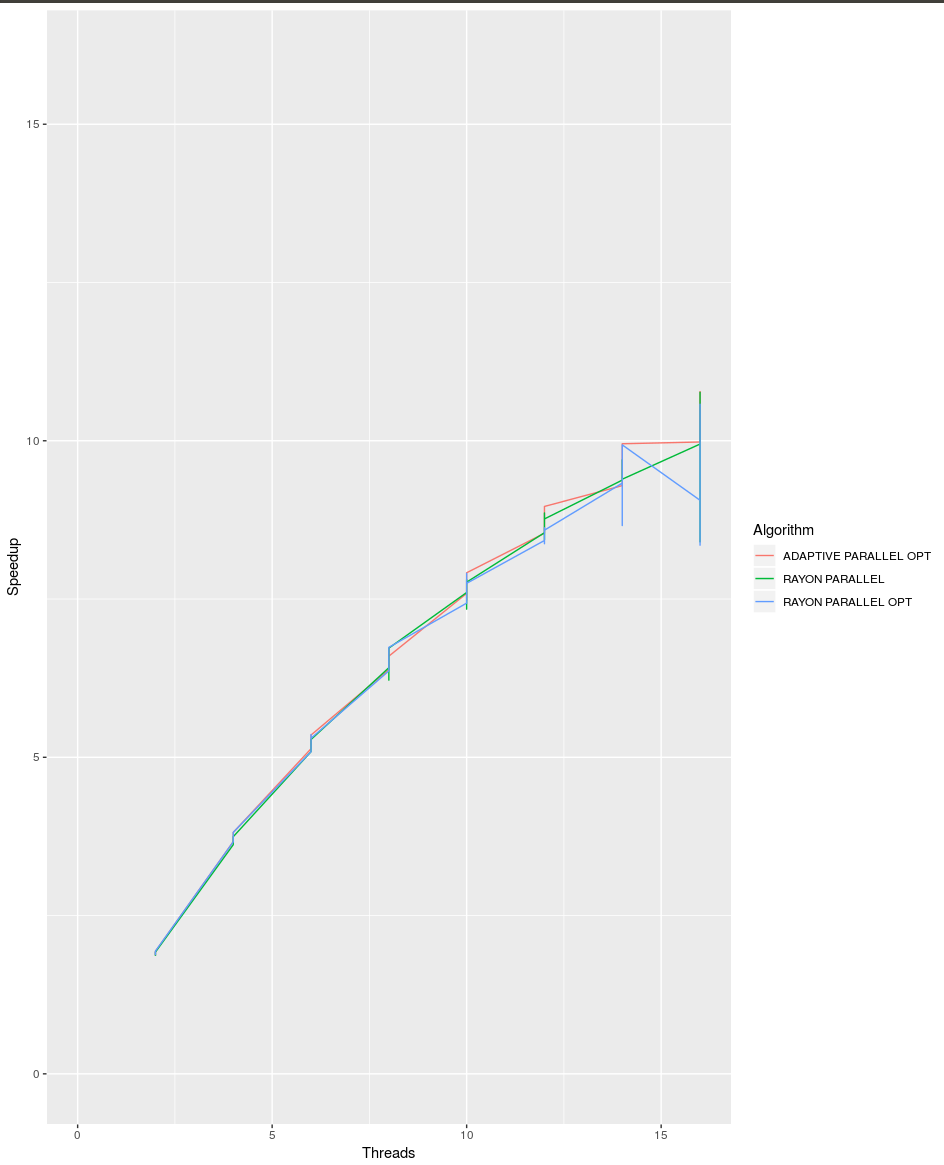
\includegraphics[scale=0.5]{Pictures/speedups.png}
	\rule{40em}{0.5pt}
    \caption[Optimization]{Speedup curves for the various parallel algorithms}
	\label{fig:speedups}
\end{figure}
The speedups were obtained as shown in Figure \ref{fig:speedups}

%----------------------------------------------------------------------------------------


